\clearpage
\chapter{\textbf{Implementation}}\label{Implementation}
\section{Sewing Machine Signal Connection and Data Acquisition}
The final signals necessary to calculate all selected KPIs are "Thread Trimming," "Pressure foot," "Upper shaft rotating," and "Main menu and not sewing." The retrieval of these signals was contingent upon their initial assignment to the correct output pins in the machine's menu configuration. The subsequent challenge was to establish a connection between the output pins and the input pins of the WAGO PLC.

A connection for one signal from the sewing machine had already been established during an earlier project, but unfortunately, the connection was inadequately documented. This proved to be more confusing than helpful. The connection was implemented as follows: The signal pin of the sewing machine was connected to the 0V reference of the PLC. The 24V pin of the sewing machine was connected to the signal input connector of the PLC. Figure 5.1 provides a visual aid to facilitate comprehension of this configuration. This arrangement made sense once it was discovered that the sewing machine signals are NPN type, while the PLC exclusively accepts PNP signals as input. Typically, when the sewing machine would also have signals of type PNP, the signal pins would simply be connected to the signal connectors of the PLC. Concurrently, the 0V connector of the PLC would be connected to the GND pin of the sewing machine.
\begin{figure}[H]
	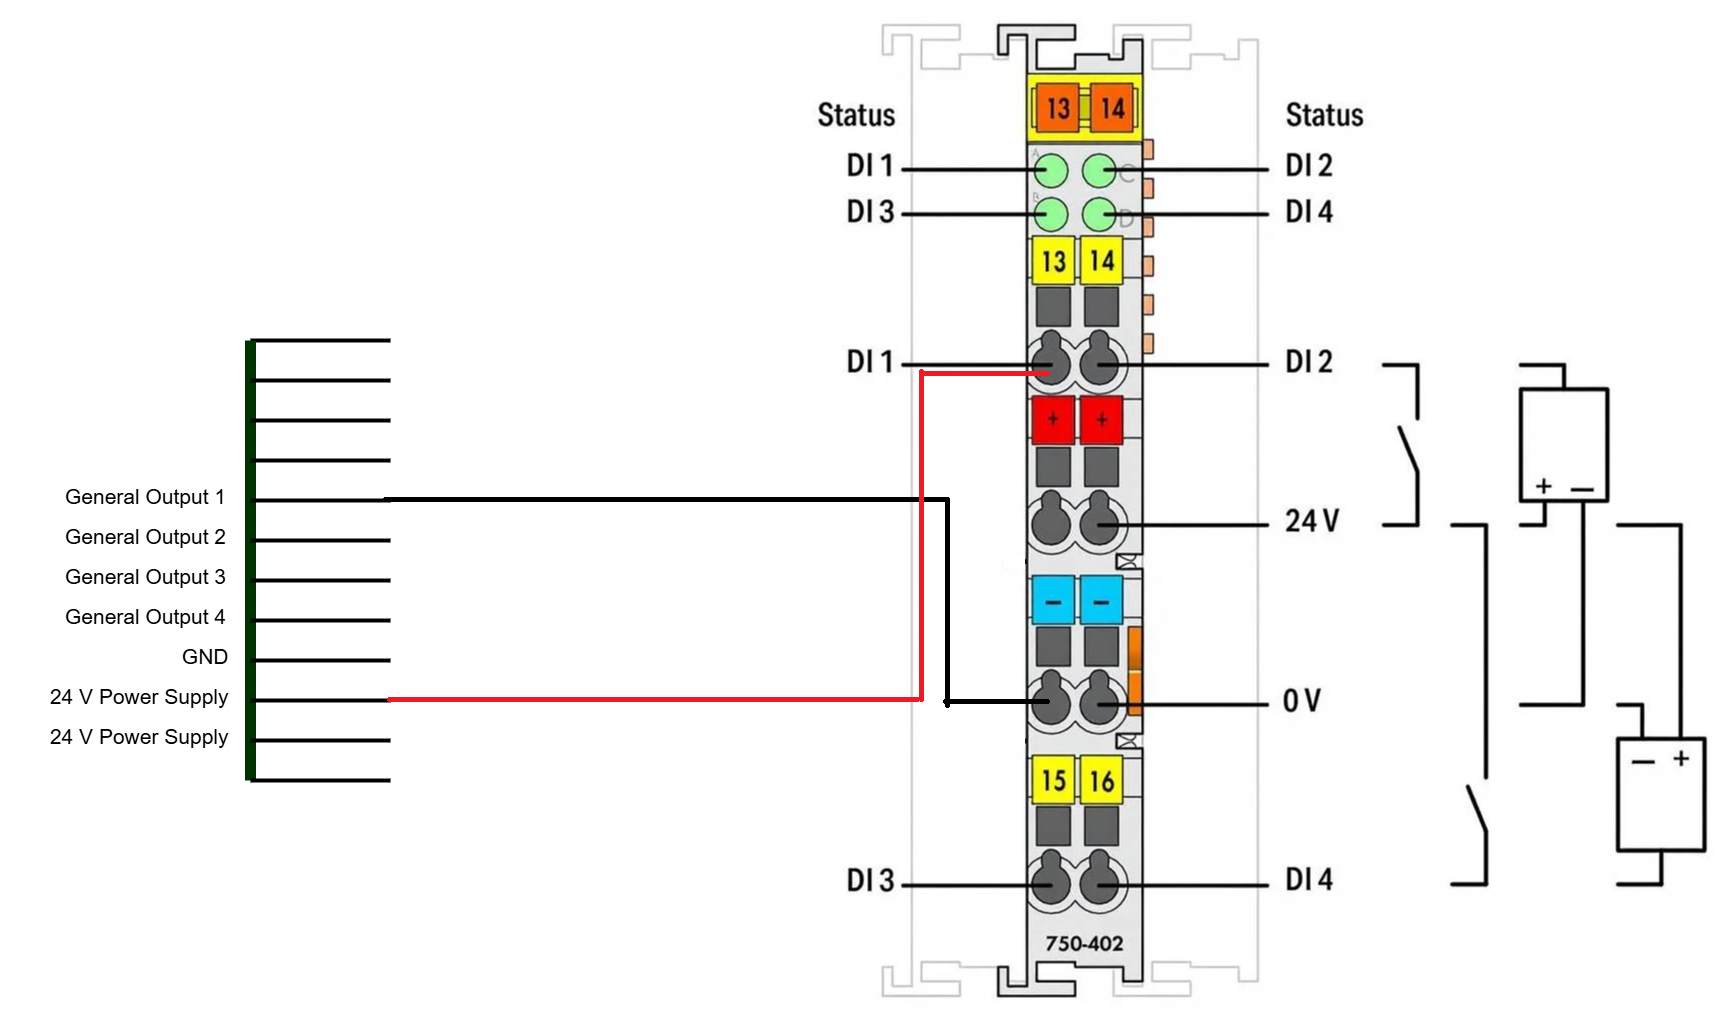
\includegraphics[height=7.4cm]{pic/sewing-machine-plc-init.png}
	\caption{Initial Connection of Sewing Machine to PLC}
	\label{fig:Model-Component-Pattern}
	\small\textit{Note: The 12-pin connector of the sewing machine is located on the left side. This connector contains various pins, including those that function as signal pins. The left side of the module contains the PLC input module. The DI1-4 marked connectors of the PLC serve the function of signal input connectors.}
\end{figure}
The system was configured so that when a signal becomes active, it draws current through the signal input connector of the PLC, resulting in a high signal. However, this implementation was limited to only two signals, because there is only one 0V connector available for two signal input connectors. In total, there are two 0V connectors and four signal input connectors. When two 24V pins are connected to one 0V connector via the signal input pins, an active signal draws current through the 0V connection and simultaneously pulls current from both input signal connectors. This results in invalid signals. 


The resolution of the aforementioned issue necessitated the conversion of the NPN signals of the sewing machine into PNP signals, which are compatible with the PLC. For the execution of this task, an optocoupler was utilized. The implementation was executed in accordance with the subsequent description. Subsequently, the signal output pins of the sewing machine were connected to the signal input connectors of the optocoupler. Furthermore, a connection to the 24-V power supply of the sewing machine was established for each signal input. The signal connectors on the output side of the optocoupler are connected to the signal input connectors of the PLC. Concurrently, the 24-V power supply of the PLC is connected to the VCC input connector of the optocoupler. Additionally, the 0V connector of the programmable logic controller PLC is linked to the GND connector of the optocoupler. The wiring of the optocoupler can be observed in the following Figure.
\begin{figure}[H]
	\centering
	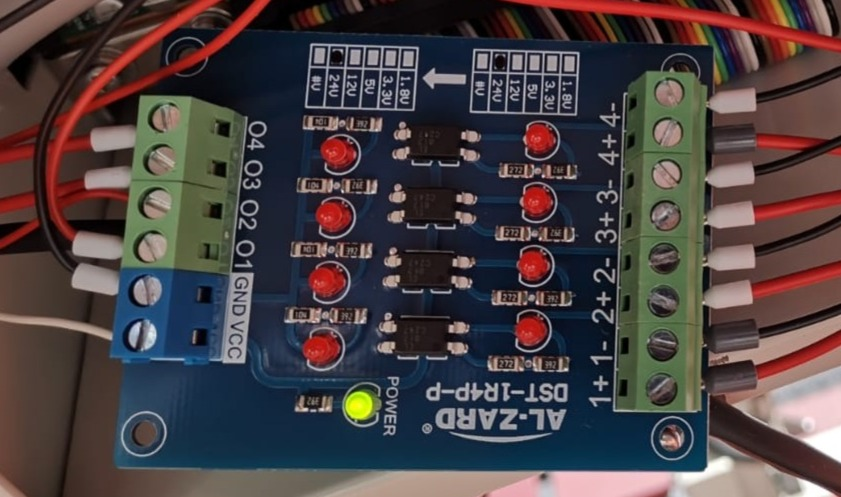
\includegraphics[height=6cm]{pic/optocoupler-wiring.jpg}
	\caption{Initial Connection of Sewing Machine to PLC}
	\label{fig:Model-Component-Pattern}
\end{figure}
As illustrated, the red cables represent electrical connections originating from or terminating at a 24V power source. Additionally, the white cable located on the left side is linked to the 24V source of the PLC. The black cables serve as connections to ground or to the signal pins on the right side. These connections function in a manner that pulls down the current when signals are in a state of activity.
In order to ensure the signal's availability across the shopfloor network, it was imperative to program the PLC in a manner that facilitated this objective. The input signals simply needed to be assigned to a value and then published over OPC UA. \\
Initially, only the IP address and the OPC UA port of the PLC were known. In order to enhance comprehension regarding the retrieval of data from the aforementioned system through the utilization of an OPC UA client, the development of a Python script was undertaken. The script under consideration took the two givens, established a connection, and navigated through the OPC UA server's node structure. The search is conducted for a "DeviceSet" node, which is understood to generally contain industrial devices, such as sewing machines. For each device identified, an exploration of its variables and child objects is initiated. It is important to acknowledge that, at this juncture, the connection from the preceding project was still in place. Further exploration was necessary to ascertain the nature of the connection and to identify any additional machines that were connected to the PLC. At this time there was a delay in communication with "Brother Internationale Industriemaschinen GmbH." Therefore, the necessary information regarding the configuration of the sewing machine signals was not available. A decision was reached to initiate an exploration of effective communication methods with the OPC UA server.\\
Subsequent to the establishment of a connection to the PLC for all signals, a diagnostic procedure was conducted to ascertain the availability of all signals. For this purpose, a tool known as UAExpert was utilized. The software under discussion is an OPC UA client that provides a user interface for development, testing, and monitoring. The device was utilized for the purpose of monitoring the values of the signals. Consequently, the actions that were expected to elicit the signals were executed on the sewing machine. Initially, the process was proceeding according to plan.

\section{Data Preprocessing}
\begin{figure}[H]
	\centering
	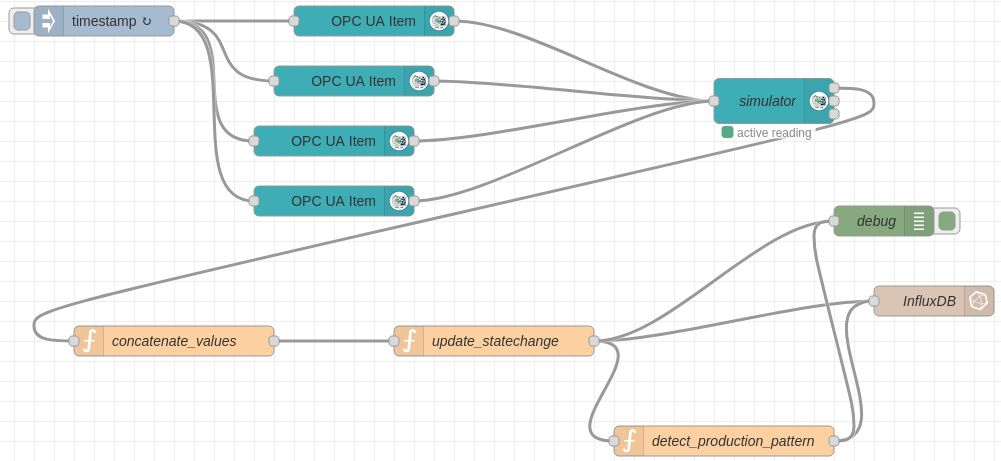
\includegraphics[height=7cm]{pic/node-RED.jpg}
	\caption{Data retrieval and preprocessing}
	\label{fig:Model-Component-Pattern}
\end{figure}
In the context of this study, Node-RED was utilized as a service to retrieve data that had been published by the PLC's OPC UA server. This feature facilitates the preprocessing and subsequent injection of data into the database. The retrieval of data from the OPC UA server is facilitated by an OPC UA package known as "node-red-contrib-opcua." The node designated as "timestamp" at the inception of the flow serves merely to initiate the flow. The temporal configuration of this feature may be set to various intervals or fixed times. The decision was made to establish an interval of 0.2 seconds. This interval was selected due to the fact that some operations on the sewing machine have an execution time of approximately one second when operated by inexperienced workers. In light of the dearth of seasoned professionals, it was deduced that an experienced worker would exhibit a fourfold increase in efficiency. To ensure the capture of all events, the interval was set to 0.2 seconds, equivalent to the execution time of a worker operating at a rate five times faster. Subsequent to the completion of the trial, the interval may be recalibrated in accordance with the findings of the evaluation. The four subsequent nodes, designated as OPC UA Items, each contain the namespace and ID of the various signals. These are subsequently fed into the simulator node. The node in question has been configured with the endpoint, which consists of the IP address of the PLC, the port, and the name of the OPC UA server, if such a server exists. This node is responsible for generating the values for each of the OPC UA items in a serial manner.
The succeeding node is one of three function nodes. These function nodes contain JavaScript code that executes three distinct preprocessing steps. The initial step involves the concatenation of the four values into a single string. The primary rationale for concatenating values is that, in InfluxDB, each value is assigned its own table. In the event that a query is executed over a set of values, the tables must be joined, a process that is computationally intensive. This phenomenon can result in substantial delays in the final dashboard. The concatenation of values eliminates the necessity for joining tables, as all values are subsequently stored within a single table.
This preprocessing step confers an additional advantage, namely that it facilitates the subsequent step in the procedure. The subsequent preprocessing step in the function node designated "update\_statechange" involves the verification of whether the concatenated string undergoes alterations. A modification in the configuration of the string is indicative of a state alteration in the sewing machine. Consequently, the string undergoes an output transformation. The initial concatenation of the values reduces the number of comparisons from four to one string. This preprocessing step was implemented to reduce the amount of data stored in the database. In previous iterations, this step was omitted, resulting in a substantial reduction in query processing speed relative to subsequent iterations. The output of the second preprocessing node is comprised of four separate key-value pairs of the signals, as well as these in a concatenated string format. It is important to note that these values are only provided as output when there is a change in one of the values compared to the previous state. The output of this node is utilized as an input for the third preprocessing node.
In the preceding section (4.0.7), the production pattern was delineated as a metric for quantifying the duration of machine utilization for value-adding operations. The final preprocessing node, designated "detect\_production\_pattern", serves to ascertain the presence of this pattern. The output of this function is the key "pattern" with a value of true, indicating the beginning of the pattern, or false, indicating the end of the pattern. Additionally, the timestamp indicating the end or beginning of the pattern is included in the output.
Upon completion of the data flow, both outputs from the "updateStateChange" function and the "detect\_production\_pattern" process are transferred to the designated InfluxDB node as input. This node has been configured with the address and the API key of the Influx database. The component in question is an InfluxDB out node, which signifies that it is capable of writing data exclusively to InfluxDB. This node stems from the node-red-contrib-influxdb package. In the course of each write operation, the system automatically incorporates a timestamp into the input. However, it is imperative to incorporate a timestamp at the "detect\_production\_pattern" node, as the pattern's detection is only possible in a retrospective manner. Consequently, the timestamp of the InfluxDB node would be inadequate.

\section{Data Storage and Post-Processing}
In the context of InfluxDB, it is necessary to establish a designated bucket for the designated project. In the context of a relational database management system (RDBMS), a bucket can be regarded as analogous to a schema. The bucket is configured with a retention policy and access rights. The retention policy is a mechanism that governs the duration for which data is retained in the bucket. The preliminary step in the process was the creation of an initial bucket, into which data was subsequently streamed from Node-RED. Initially, an unlimited retention policy was configured for the specified bucket. Subsequently, in light of apprehensions pertaining to an excess of data, the determination was made to curtail the retention policy to a span of one day. Following the initialization of the process, the data of the first bucket is aggregated and stored in a separate bucket that employs an unlimited retention policy. The aggregation process leads to a substantial reduction in the amount of data that must be stored. Aggregation is performed within designated tasks. These tasks can be configured to execute either upon the completion of a specified time interval or through the utilization of cron syntax, which facilitates the establishment of a predetermined time for regular aggregation. The latter is employed in this implementation. The rationale underlying this necessity is that it is imperative for the aggregation to occur during the period between the conclusion of one shift and the commencement of the subsequent one. This phenomenon can be attributed to the prevalence of data aggregation processes that are contingent upon the identification of the initial and concluding points of an event. In the case that the aggregation occurred between these events, the result would be a falsification. The aggregation could also be executed at eight-hour intervals, thereby aligning with the duration of a typical shift. However, given the legal framework delineated in the foundational chapter, the daily aggregation is applied. The implementation of an eight-hour aggregation period would result in the accumulation of data that could be traced back to a specific worker. The aggregation of data over the course of an entire day encompasses three shifts. Consequently, it is not possible to draw any conclusions from the data regarding the individual performance of a worker. A notable benefit of this approach is a significant reduction in the necessary storage capacity, amounting to approximately two-thirds of the original requirement.
The aggregation of these data is facilitated by the utilization of the flux query language. Throughout the developmental process, the aggregations were meticulously formulated in flux notebooks. These notebooks bear a resemblance to Jupyter notebooks and can be utilized within the web user interface of the InfluxDB DBMS. Cells for flux queries and additional cells for visualizing the result or displaying the resulting table(s) can be added to the notebook. In this manner, the proper functioning of the query can be readily corroborated. A thorough exposition of the methodology employed for the verification of results can be found in the Evaluation chapter. The results of the aggregations encompass all of the supporting elements.

\subsection{Flux Query Language}
\begin{lstlisting}[style=FluxStyle, caption={Flux aggregation query for produced quantity}]
from(bucket: "sewing-machine-1-simulated")
|> range(start: -24h)
|> filter(fn: (r) => r["_measurement"] == "sewingMachine1")
|> filter(fn: (r) => r["_field"] == "thread_trimming" and r["_value"] == true)
|> count()
|> map(fn: (r) => ({r with _time: now()}))
|> map(fn: (r) => ({r with _field: "pieces"}))
|> to(bucket: "simulated-tasks")
\end{lstlisting}
A comparison of the flux query language with SQL-like query languages reveals notable distinctions in their respective syntax and semantics. Accordingly, the fundamental principles of flux querying are elucidated herein. The initial step in the process is the selection of the bucket from which the data is to be utilized for processing, as illustrated in the initial row. The "|>" (pipe forward) symbol is employed in each subsequent row. This operator indicates that the result of the preceding operation is to be utilized in the subsequent operation. The subsequent row is designated for the specification of the timeframe for the desired data. This is a common practice at the outset to minimize data and, consequently, processing time. Furthermore, the subsequent filtration operations function in a similar manner, thereby allowing for the selection of only the pertinent data. The "\_measurement" constitutes a logical grouping of the data, encompassing numerous tags and fields. The utilization of tags facilitates the creation of additional data groups. For instance, in the event that a project encompasses multiple sewing machines, the measurement name could be altered to "State," and the tag could contain the names of the identifiers for each sewing machine.  Fields are defined by a name and a value, and their distinguishing characteristic is that they undergo changes over time. Subsequent processing of the data typically occurs subsequent to the filtration stage. The number of operations that can be chained together is unlimited. The count operation in this particular instance is one of numerous aggregate functions that reduce the quantity of values to a single value. The map function can be used to apply a function to every row in a data set. Upon completion of the query, the final result is returned. In this particular instance, the result is written to an alternate bucket.

\subsection{Postprocessing Task Queries}
This subsection briefly explains how aggregations of all supporting elements are queried.

\textbf{Processed Quantity}\\
The sum of all thread trimming events where the value is true is being calculated.

\textbf{Actual Downtime}\\
Downtime events are determined by summing idle or machine-off times that exceed a set threshold. Keep in mind that sometimes a worker goes to the bathroom or takes a short break. Initially, the threshold was set to ten minutes. Then, it is filtered for all events where all signals except "main\_menu\_not\_sewing" are false. The latter can be true (idle) or false (machine off). All remaining entries above the threshold are summed up.

\textbf{Actual Production Time}\\
The sum of all event durations where the pattern tag is true is being calculated.

\textbf{Actual Cycle Time}\\
The duration between two cycle times is measured and summed up. To ensure that no breaks or downtime events are included, the same threshold used for the downtime measurement is applied to filter the values.

\textbf{Setup Time}\\
The time from when the machine is turned off until the first sewing event is measured and summed up for each shift of the day. A machine is considered off when all signals have the value false. A sewing event is characterized by only the "sewing\_active" signal being true.

\textbf{Idle Time}\\
The duration of all events in which all signals except "main\_menu\_not\_sewing" are false is measured and summed up. Then, the duration of the break is subtracted. Of course, these events could still contain downtime events. However, downtime is simply subtracted in later queries.

\textbf{Failure Events}\\
All events in which all signals are false, except for "main\_menu\_not\_sewing," which can be either true or false, are filtered out. Then, the threshold filter is applied again. Finally, the number of events is counted.\\

The remaining maintenance elements were omitted because they depend on some of the supporting elements, such as actual downtime and production time. None of the supporting elements that are "planned" were mentioned because they cannot be queried, only defined.

\section{Synthetic Data Generation}
The implementation follows a staged approach to data generation and validation. Phase 1 employs offline synthetic datasets to design KPIs and to verify computations against ground truth. Phase 2 uses an online simulator via an OPC UA mock to evaluate streaming behavior, end-to-end latency, and storage characteristics. Phase 3 targets on-machine integration. This approach decouples progress from hardware availability, enables controlled experiments with ground truth, and preserves reproducibility through fixed seeds and configurable scenarios.
For phase 1, a Python script was developed. At the inception of the script, a series of parameters were established. The parameters in question encompass the duration of the shift, the number of hours that elapse before the commencement of the break, the duration of the break itself, the timeframe of the simulated data, and the step width with which the data is generated. In an effort to emulate the actual production process, it was determined that random values would be employed for various parameters, including setup times, idle times, sewing times, breakdown durations, and the number of breakdowns. For these random values, upper and lower limits were established at the outset. The data that was generated has the following structure. A period of inactivity occurs between each shift, during which the worker is responsible for setting up the machine and readying the workplace. This segment of time is considered to be "idle." Subsequently, the pattern delineated in Chapter 4.7 is reiterated in sporadic intervals. An idle event occurs between each step of the pattern because, under normal circumstances, the time frame for observing the pattern on a millisecond time scale invariably includes a period of inactivity between each action. Occasionally, intervals of downtime coincide with the patterns. Also one lunch break is included in each shift. In the script, the initial step entails the creation and subsequent storage of the data as a CSV file on a daily basis. Subsequently, it undergoes a transformation into the InfluxDB line protocol, and is then written in batches to the database.
In the second phase, two Python scripts were implemented. The first is nearly indistinguishable from the script from phase 1. The generated data is almost identical to that of the original, with only minor variations, and is subsequently written to a CSV script. A salient distinction is that the data is populated to emulate a continuous stream of data analogous to that of the sewing machine. The filling up is realized through utilization of the forward fill method. This method utilizes a two-step process to address the aforementioned issues. First, it employs a technique that utilizes the previous state of the system to fill in the missing data. Second, it generates values based on the sampling rate. The generation of a new CSV file occurs at the 24-hour interval, thereby encompassing the subsequent 24-hour period. To ensure a sufficient supply of data, the process of data generation is initiated several hours prior to the timestamp of the most recent data entry within the previous 24-hour period. The second script utilizes the CSV file, initiates an OPC UA server, and streams the data at the designated sampling rate. The construction of the system is such that initiation is permitted at any point in time. The efficacy of this method is predicated on its ability to identify the entry that is temporally closest to the current time.


\section{Infrastructure Automation and Service Health}
The final system was designed to operate on a server equipped with the Fedora Linux operating system. In order to ensure a seamless deployment experience, particularly for colleagues who may repeatedly utilize the solution, it was determined that Docker should be employed as the orchestration tool of choice. A favorable consequence of this was that the development of the solution could be readily executed on various machines. The orchestration process was facilitated by the implementation of a Docker Compose YAML file. With the exception of the "simulator," for each service, the data and config folders were mounted to the data and config folders, respectively, within the project folder. This modification enabled the versioning of contents within folders. In the context of Node-RED, the InfluxDB API token was configured due to its transient nature when configured within the web user interface. A health check was configured for InfluxDB due to its propensity for crashing. Upon exiting, the container is restarted. A watchdog script has been implemented to facilitate the exit of the container when it becomes unhealthy. It has been established that Grafana and Node-RED are contingent upon InfluxDB, necessitating a delay in their initiation until InfluxDB is operational. The fourth container is the simulator. The system under consideration simulates real-time data flow from the sewing machine. Due to the composition of two scripts, an additional supervisor configuration was implemented to orchestrate the order of execution. This necessity arises from the interdependence between the two scripts.
Given the necessity of additional packages in Node-RED, it is imperative to execute a command during the deployment process to facilitate the installation of these packages. In addition, it was determined that there are issues with access rights on Linux machines. In order to circumvent the necessity of addressing these issues in the event of each new start script, it was deemed a prudent course of action to implement a more systematic approach. The solution contains all the necessary commands to successfully initiate it. Consequently, when the solution is implemented in a different system or modifications are being made, it is sufficient to execute only the start script to initiate all containers.
The versioning of the entire system is performed in GitLab. In the context of Docker images, it is imperative to emphasize that only the data and configuration files, in conjunction with the delineated scripts and Docker (compose) files, necessitate versioning. This approach has been demonstrated to result in a substantial reduction of overhead expenditures.

